% cSpell: disable
\section{Going even deeper}

\begin{frame}[plain,c]
    %\frametitle{A first slide}

    \begin{center}
        \color{DarkBlue}
    \Huge \thesection. \insertsection
    \end{center}

\end{frame}


\begin{frame}{Why should we go deep?}
    % with deeper models, comes better performance
    % figure of Pezzotti et al.
    % The general empirical gist of DL is that with deeper models comes better performance.
    With deeper models comes better performance.
    \begin{figure}
        \begin{overprint}
            \onslide<2>\centering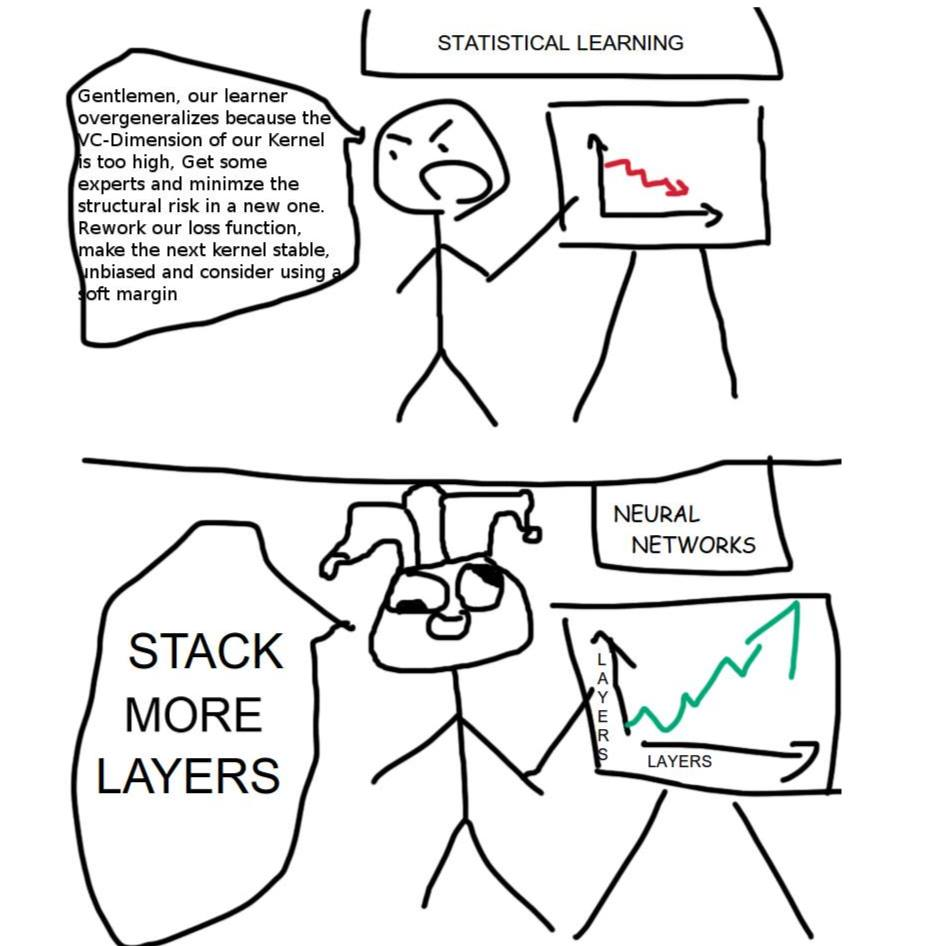
\includegraphics[width=0.4\textwidth]{Figures/shine_figures/more_layers.jpg}\caption{Credits: \href{reddit.com/r/ProgrammerHumor/comments/5si1f0/machine_learning_approaches/}{reddit.com/r/ProgrammerHumor/comments/5si1f0/machine\_learning\_approaches/}}
            \onslide<3>\centering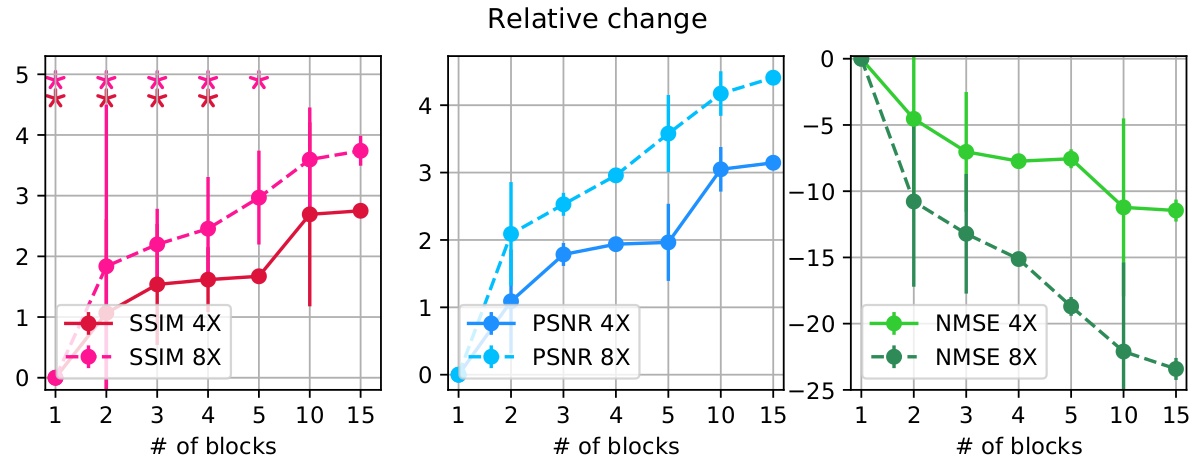
\includegraphics[width=0.78\textwidth]{Figures/shine_figures/pezzotti.png}\caption{\textbf{Performance of an unrolled MRI reconstruction network function of the number of iteration units (blocks).}\footnotemark}
        \end{overprint}
    \end{figure}
    \vspace{-4em}
    \only<3>{\footnotetext{\fullcite{Pezzotti2020AnReconstruction}}}
\end{frame}

\begin{frame}{Can we go deeper?}
    % in the current state not: activations + constrained memory
    % The big problem at hand is that deeper models need more \textbf{memory} to train, and the memory we have is constrained.
    Deeper models $\Rightarrow$ more \textbf{memory} to train.
    Memory we have is constrained.
    \pause

    % This memory requirement comes primarily from the \textbf{activations} of the model, not from the model weights.
    Why more memory? \textbf{Activations}!
    \pause

    \tikzset{%
        highlight_act/.style={rounded rectangle, draw=red!67, dashed, inner sep=0.03em, visible on=<5>},
    }


    \begin{center}
        \begin{tikzpicture}[
            font=\Large, node distance=2.5em,>=stealth,
            function/.style={circle,draw},
        ]
            % nodes
            \begin{scope}[execute at begin node=$, execute at end node=$]
                \node (input_node) {\xb};
                \node (first_int_function) [right=of input_node, function] {f_{\thetab_1}};
                \node (dots) [right=of first_int_function] {\ldots};
                \node (last_int_function) [right=of dots, function] {f_{\thetab_N}};
                \node (output_node) [right=of last_int_function] {\hat{\yb}};
            \end{scope}

            % arrows
            \draw[->] (input_node) -- (first_int_function);
            \draw[->] (first_int_function) -- (dots) node (first_activation) [above,midway] {$\zb_1$};
            \draw[->] (dots) -- (last_int_function) node (last_activation) [above,midway] {$\zb_{N-1}$};
            \draw[->] (last_int_function) -- (output_node);

            % highlights
            \node (highlight_first_activation) [highlight_act, fit=(first_activation)] {};
            \node (highlight_last_activation) [highlight_act, fit=(last_activation)] {};


        \end{tikzpicture}
    \end{center}

    \pause
    \begin{equation*}
        \frac{\partial \mathcal{L}}{\partial \thetab_1} = \frac{\partial \mathcal{L}}{\partial \hat{\yb}}\Bigr|_{\hat{\yb}} \; \frac{\partial \hat{\yb}}{\partial \zb_{N-1}}\Bigr|_{\tikzmarknode[highlight_act]{last_eq_activation}{\zb_{N-1}}} \; \ldots \; \frac{\partial \zb_2}{\partial \zb_1}\Bigr|_{\tikzmarknode[highlight_act]{first_eq_activation}{\zb_1}} \; \frac{\partial \zb_1}{\partial \thetab_1}\Bigr|_{\thetab_1}
    \end{equation*}

\end{frame}

\begin{frame}{The modeling solutions}
    % gradient checkpointing
    % Invertible networks
    % Implicit models
    % On the modeling side, several solutions exist:
    Memory-efficient training:
    \begin{itemize}[<+->]
        \item gradient checkpointing~\citep{Chen2016TrainingCost}
        \item invertible networks~\citep{Gomez2017TheActivations,Sander2021MomentumNetworks}
        \item \highlight{blue}{implicit models~\citep{Chen2018NeuralEquations,Bai2019DeepModels}}
    \end{itemize}
\end{frame}

\begin{frame}{Infinite depth neural networks}
    A recurrent expression of classical, explicit networks:
    \only<1>{
        \begin{center}
            \begin{tikzpicture}[
                font=\Large, node distance=2.5em,>=stealth,
                function/.style={circle,draw},
            ]
                % nodes
                \begin{scope}[execute at begin node=$, execute at end node=$]
                    \node (input_node) {\xb};
                    \node (first_int_function) [right=of input_node, function] {f_{\thetab_1}};
                    \node (dots) [right=of first_int_function] {\ldots};
                    \node (last_int_function) [right=of dots, function] {f_{\thetab_N}};
                    \node (output_node) [right=of last_int_function] {\hat{\yb}};
                \end{scope}

                % arrows
                \draw[->] (input_node) -- (first_int_function);
                \draw[->] (first_int_function) -- (dots) node (first_activation) [above,midway] {$\zb_1$};
                \draw[->] (dots) -- (last_int_function) node (last_activation) [above,midway] {$\zb_{N-1}$};
                \draw[->] (last_int_function) -- (output_node);

            \end{tikzpicture}
        \end{center}

    }
    \only<2->{
        \begin{equation*}
            \zb_{n} = f_{\thetab_{n}}(\zb_{n-1}), \quad \forall n < N
        \end{equation*}
    }

    \onslide<3->{
        What if $N \to \infty$?
    }


\end{frame}

\begin{frame}{Deep Equilibrium networks - 1}
    % give equation and how to compute the gradient with IFT
    % \citet{Bai2019DeepModels} introduced \textbf{Deep Equilibrium networks~(DEQs)}, a type of implicit model.
    \textbf{Deep Equilibrium networks~(DEQs)}~\citep{Bai2019DeepModels} are a type of implicit model.
    % The output of DEQs is defined implicitly as the solution to a fixed-point equation.
    The output is the solution to a fixed-point equation.

    \begin{equation*}
        h_{\thetab}(\xb) = \zb^\star, \text{ where } \alt<3>{g_\thetab(\zb^\star, \xb) = \zb^\star - f_\thetab(\zb^\star, \xb) = 0}{\zb^\star = f_\thetab(\zb^\star, \xb)}
    \end{equation*}

    \pause

    % In practice, we solve this equation with a \textbf{quasi-Newton method}.
    In practice, solved with a \textbf{quasi-Newton method}.
\end{frame}

\begin{frame}{Deep Equilibrium networks - 2}
    % The big question is now: how do I compute the gradient $\frac{\partial \mathcal{L}}{\partial \thetab}$?
    How do I compute the gradient $\frac{\partial \mathcal{L}}{\partial \thetab}$?
    \pause

    The \textbf{Implicit Function Theorem} gives us just that:
    \begin{theorem}[Hypergradient~\citep{Krantz2013TheApplications,Bai2019DeepModels}]
        Let $\thetab \in \mathbb{R}^p$ be a set of parameters, let $\mathcal{L}: \mathbb{R}^d \rightarrow \mathbb{R}$ be a loss function and $g_{\thetab}: \mathbb{R}^d \rightarrow \mathbb{R}^d$ be a root-defining function.
Let $\zb^\star \in  \mathbb{R}^d$ such that $g_{\thetab}(\zb^\star) = 0$ and $J_{g_{\thetab}}(\zb^\star) = \frac{\partial g_{\theta}}{\partial \zb}\Bigr|_{\zb^\star}$ is invertible, then the gradient of the loss $\mathcal{L}$ wrt. $\thetab$, called Hypergradient, is given by
\begin{equation*}
    \frac{\partial \mathcal{L}}{\partial \thetab}\Bigr|_{\zb^\star} = \tikzmarknode[rounded rectangle, draw=red!47, dashed, inner sep=0.1em]{grad_no_act}{\nabla_\zb \mathcal{L}(\zb^\star)^\top J_{g_{\thetab}}(\zb^\star)^{-1} \frac{\partial g_{\thetab}}{\partial \thetab}\Bigr|_{\zb^\star}} \, .
\end{equation*}
    \end{theorem}
    % Key for our memory problem: it does not rely on any activations you could have when solving the fixed-point equation.
    \begin{tikzpicture}[overlay,remember picture,>=stealth,nodes={inner ysep=1pt},<-]
        % For "aliased_image"
        \onslide<3>{
        \path (grad_no_act.south) ++ (0, -2em) node[anchor=north,color=red!47] (exp){
            Does not rely on activations!};
            \draw [color=red!47](grad_no_act.south) -- ([color=red]exp.north);
        }
    \end{tikzpicture}
\end{frame}

\begin{frame}{The limits of DEQs}
    % they are slow to train
    DEQs achieve excellent results in NLP~(Natural Language Processing) and CV~(Computer Vision) tasks, but they are slow to train.

    \begin{figure}
        \centering
        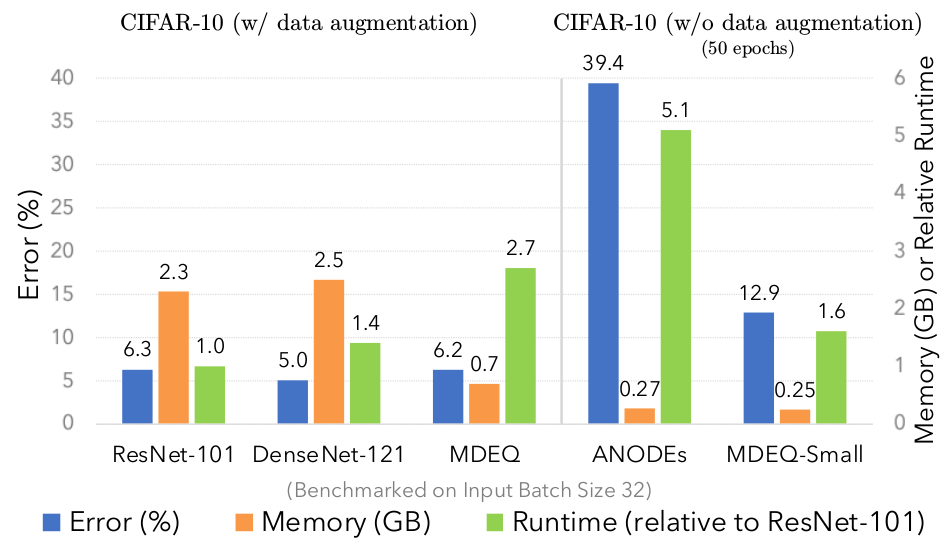
\includegraphics[width=0.6\textwidth]{Figures/shine_figures/deq_memory.png}
        \caption{\textbf{Performance, memory and training speed of DEQs.}~\citep{Bai2020MultiscaleModels}}
    \end{figure}
    \let\thefootnote\relax\footnotetext{
        DEQs: Deep Equilibrium Networks
    }
\end{frame}

\begin{frame}{Why are DEQs slow?}
    % bc of Jacobian inversion
    % If we look back the equation used to compute the gradient of DEQs:
    DEQs gradient computation:
    \begin{equation*}
        \frac{\partial \mathcal{L}}{\partial \thetab}\Bigr|_{\zb^\star} = \highlight{green}{$\nabla_\zb \mathcal{L}(\zb^\star)^\top$} \highlight{red}{$J_{g_{\thetab}}(\zb^\star)^{-1}$} \frac{\partial g_{\thetab}}{\partial \thetab}\Bigr|_{\zb^\star} \, ,
    \end{equation*}
    % we see that we need to invert a huge matrix \highlight{red}{$J_{g_{\thetab}}(\zb^\star)$} in a certain direction \highlight{green}{$\nabla_\zb \mathcal{L}(\zb^\star)$}.
    we need to invert a huge matrix \highlight{red}{$J_{g_{\thetab}}(\zb^\star)$} in a certain direction \highlight{green}{$\nabla_\zb \mathcal{L}(\zb^\star)$}.
    \pause

    In practice this is done using an iterative algorithm.

    \let\thefootnote\relax\footnotetext{
        DEQs: Deep Equilibrium Networks
    }
\end{frame}

\begin{frame}{Can we avoid the Jacobian inversion?~[Ramzi et al. 2022b]}
    % yes: reuse a by-product of the forward pass, share the inverse estimate
    \begin{exampleblock}{Contribution \#4}
        \fullcite{Ramzi2021_shine}
    \end{exampleblock}

    We introduced \textbf{SHINE: SHaring the INverse Estimate}.

    \begin{equation*}
        \tikzmarknode{qn_matrix}{\highlight{blue}{$\Bb^{-1}$}} \approx \tikzmarknode{true_jacobian}{\highlight{red}{$J_{g_{\thetab}}(\zb^\star)^{-1}$}}
    \end{equation*}

    \begin{tikzpicture}[overlay,remember picture,>=stealth,nodes={align=left,inner ysep=1pt},<-]
        % For "kspace"
        \onslide<2->{
        \path (true_jacobian.south) ++ (0,-2em) node[anchor=south west,color=red!87] (exp_jac){
            \textbf{True Jacobian inverse}};
        \draw [color=red!87](true_jacobian.south) |- ([xshift=-0.3ex,color=red]exp_jac.south east);
        }
        % For "image"
        \onslide<3->{
        \path (qn_matrix.south) ++ (0, -2em) node[anchor=south east,color=blue!87] (exp_qnm){
            \textbf{quasi-Newton matrix}};
        \draw [color=blue!87](qn_matrix.south) |- ([xshift=-0.3ex,color=blue]exp_qnm.south west);
    }
    \end{tikzpicture}
    \pause

    \hfill \break
    \begin{overprint}
        \onslide<4-5>
        Properties of \highlight{blue}{$\Bb$}:
    \begin{itemize}
        \item<4-> It is computed when solving $g_\thetab(\zb^\star, \xb) = 0$ using a quasi-Newton method.
        \item<5-> It is easily invertible using the Sherman-Morrison formula, because low-rank.
    \end{itemize}


    \onslide<6>
        We have asymptotic correctness of the approximation!
    \end{overprint}


\end{frame}

\begin{frame}{Computer vision results~[Ramzi et al. 2022b]}
    \begin{figure}
        \centering
        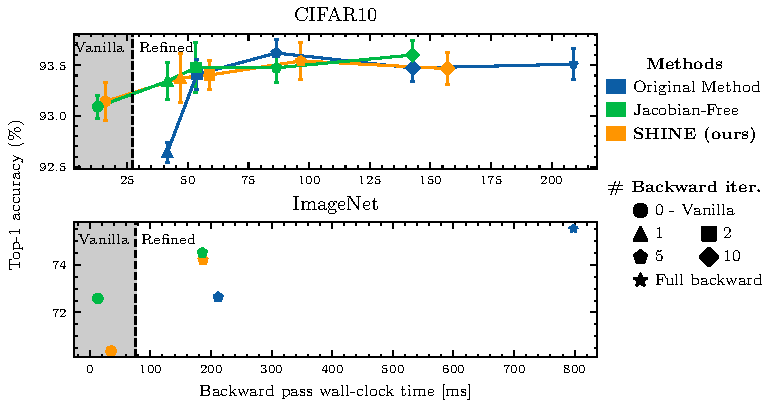
\includegraphics[width=0.8\textwidth]{Figures/shine_figures/merged_results_latency_style.pdf}
        \caption{\textbf{MDEQs~\citep{Bai2020MultiscaleModels} with SHINE.}}
    \end{figure}
\end{frame}

\begin{frame}{Application to Hyperparameter optimization - 1 [Ramzi et al. 2022b]}
    % it's also a bilevel prob
    % Interestingly, other problems can benefit from this idea, notably Hyperparameter optimization.
    Hyperparameter optimization can benefit from SHINE.

    \begin{equation*}
        \begin{split}
            &\argmin_{\lambda} \mathcal{L}_{\text{val}}(\xb^\star)\\
            \text{s.t. } \quad \xb^\star = &\argmin_{\xb} \mathcal{L}_{\text{train}}(\xb) + \exp^{\lambda} \|\xb\|_2^2
        \end{split}
    \end{equation*}

    \pause
    The IFT can also be applied, and when a quasi-Newton method is used to solve $\argmin_{\xb} \mathcal{L}_{\text{train}}(\xb) + \exp^{\lambda} \|\xb\|_2^2$, we may use SHINE.
\end{frame}

\begin{frame}{Application to Hyperparameter optimization - 2 [Ramzi et al. 2022b]}
    \begin{figure}
        \centering
        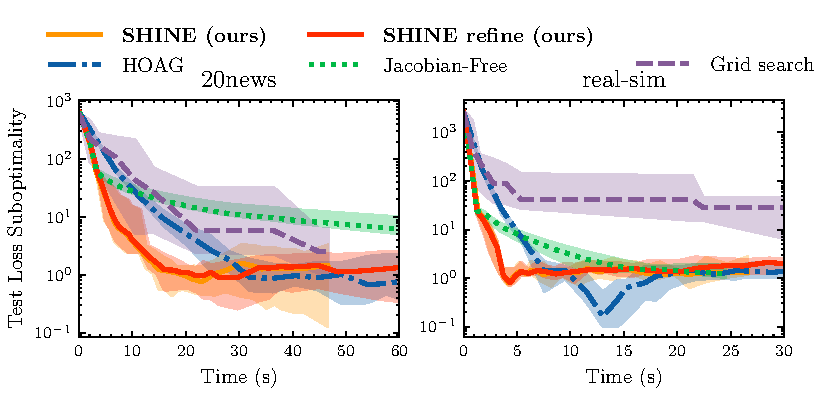
\includegraphics[width=0.85\textwidth]{Figures/shine_figures/bilevel_test.pdf}
        \caption{\textbf{Bilevel optimization~\citep{Pedregosa2016HyperparameterGradient} with SHINE:} convergence of held-out test loss.}
    \end{figure}

\end{frame}

% \begin{frame}{SHINE}
%     \begin{block}{Recap}
%         MRI is slow because of \textbf{relaxation}.

%         \pause
%         If we want to do fewer relaxations, we need to exploit some \textbf{redundancy} in MR images.

%         \pause
%         \textbf{Deep Learning} allows us to learn more complex structures in MR images than Compressed Sensing.

%         \pause
%         But if we want to get the best performance, we need deep memory-hungry models.
%         \textbf{DEQs} are a solution to the memory requirements but are slow to train.
%         We introduced a method that could enable faster DEQ training.
%     \end{block}
% \end{frame}
